\documentclass{article}

\usepackage[paperwidth=190mm,paperheight=330mm, margin={.5in,.6in}]{geometry}
% \usepackage[a4paper, margin={.5in,1in}]{geometry}
\usepackage{amsmath}
\usepackage{mathdots}
\usepackage{tikz}
\usetikzlibrary{arrows,matrix,positioning}
\usetikzlibrary{fit}

\newcommand{\tr}{\operatorname{tr}}
\newcommand{\rank}{\operatorname{rank}}
\newcommand{\diag}{\operatorname{diag}}


% :syntax match texMathSymbol "\\A" conceal cchar=A
% :syntax match texMathSymbol "\\B" conceal cchar=B
% :syntax match texMathSymbol "\\I" conceal cchar=I
\newcommand{\A}{\boldsymbol{A}}
\newcommand{\B}{\boldsymbol{B}}
\newcommand{\I}{\boldsymbol{I}}

\begin{document}

\section{Trick}

\subsection{Test for linear independence when finding eigenvalues}

\[
\begin{vmatrix}
\ddots & \vdots & \vdots     & \vdots & \vdots & \vdots & \vdots \\
\cdots &        & a          & b      &        &       &        \\
\cdots & d      & g -\lambda & c      &        &        &        \\
\cdots & e      & f          &        &        &        &        \\
\cdots &        &            &        &        &        &        \\
\cdots &        &            &        &        &        &        \\
\cdots &        &            &        &        &        &        \\
\end{vmatrix}
\] 

When trying to find eigenvalues, we hope $|\A-\lambda\I|=0$, and this happens
when two rows (or columns) are linearly dependent. As shown above, if we can find
$\lambda$ such that  \[
\begin{vmatrix}
	a & b \\
	g-\lambda & c \\
\end{vmatrix}=0\quad \text{or}\quad
\begin{vmatrix}
 d & g-\lambda \\
 e & f \\
\end{vmatrix}=0
\] 
then the whole determinant is zero, thus we find one eigenvalue. And this 2 order
determinant equation is easy to solve. We can get:
\[
	\begin{align}
	\lambda_{\text{test1}} = \frac{ac-bg}{-b} = \frac{
		\begin{vmatrix}
			a & b \\
			g & c \\
		\end{vmatrix}
	}{-b} \\
	\lambda_{\text{test2}} = \frac{df-eg}{-e} = \frac{
		\begin{vmatrix}
			d & g \\
			e & f \\
		\end{vmatrix}
	}{-e} \\
	\end{align}
\] 
And when one of $g$ surround elements($a,c,f,d$) is zero, the test eigenvalue is
directly  $g$


\section{Determinant}

\[
	\begin{align}
		\begin{vmatrix}
			a_{11} & a_{12} & \dots & a_{1n} \\
			a_{21} & a_{22} & \dots & a_{2n} \\
			\vdots & \vdots & \ddots & \vdots \\
			a_{n1} & a_{n2} & \dots & a_{nn} 
		\end{vmatrix}
		&= \sum_{\sigma \in S_n} \text{sgn}(\sigma) \prod_{i=1}^n a_{i, \sigma(i)} \\
		&= \sum_{j_1j_2\cdots j_n} (-1)^{\tau(j_1j_2\cdots j_n)} a_{1j_1} a_{2j_2} \cdots a_{nj_n}
	\end{align}
\] 

\[
	\begin{align}
	|kA| = k^n |A| \\
	|A^{*}| = |A|^{n-1} \\
	\end{align}
\] 

Row or column elements times their cofactors sum to the determinant, 
times otherwise zero:
\[
	\sum_{k=1}^{n} a_{ik} A_{jk} = |A| \delta_{ij}
\] 
\[
	\sum_{k=1}^{n} a_{ki} A_{kj} = |A| \delta_{ij}
\] 
\subsection{Important determinants}

upper/lower triangular:
\[
	|A| = \prod_{i=1}^{n} a_{ii}
\]
upper-left/lower-right triangular:

\[
A=
\begin{vmatrix}
	a_{11} & a_{12} & \dots & a_{1n} \\
	a_{21} & a_{22} & \iddots & 0\\
	\vdots & \iddots & \iddots & \vdots \\
	a_{n1} & 0 & \dots & 0
\end{vmatrix}
= (-1)^{\frac{n(n-1)}{2}}\prod_{i=1}^{n} a_{i, n-i+1}
\]
for small n values we have

\begin{itemize}
 \item 2,3 order sgn: -1
 \item 4,5 order sgn: +1
\end{itemize}

\subsection{Special determinants}

\subsubsection{ two slash one star}

use definition their only has two non-zero chooses, or use cofactor expansion directly

\[
	\begin{vmatrix}
		1 & 5 &   &   \\
      & 2 & 6 &   \\
      &   & 3 & 7 \\
		8 &   &   & 4 \\
	\end{vmatrix}
	= (-1)^{\tau_1} 1\times2\times3\times4 + (-1)^{\tau_2} 5\times6\times7\times8

\] 

\subsubsection{$|\overline\backslash$ shape}

use column operation to eliminate first column to get upper triangular
\[
\begin{vmatrix}
	1 & 2          & 3          & 4 \\
	2 & 1          &            &   \\
	3 & \leftarrow & 1          &   \\
	4 & \leftarrow & \leftarrow & 1 \\
\end{vmatrix}
=
\begin{vmatrix}
	k  & 2 & 3 & 4 \\
	 0 & 1 &   &   \\
	0  &   & 1 &   \\
	0  &   &   & 1 \\
\end{vmatrix} = k
\] 

where $k=1-2^2-3^2-4^2$

\subsubsection{bow shape}
use column operation to eliminate first row to get simple form can use cofactor expansion
\[
\begin{vmatrix}
	1 & 1 & 1 & 1 \\
	2 & \leftarrow &\leftarrow  & 2 \\
	3 & \leftarrow & 3 &  \\
	4 & 4 &  &  \\
\end{vmatrix}
=
\begin{vmatrix}
	k & 1 & 1 & 1 \\
	0 &  &  & 2 \\
	0 &  & 3&  \\
	0 & 4 &  &  
\end{vmatrix} = (-1)^{\tau} k \times 2 \times 3 \times 4
\] 
where $k=1-1-1-1$

\subsubsection{two slash one line}

use one slash to eliminate other slash
\[
\begin{vmatrix}
	 &  & -1 & 2 \\
	 & -1 & 2 &  \\
	-1 & 2 &  &  \\
	4 & 3 & 2 & 1 \\
\end{vmatrix}
=
\begin{vmatrix}
	 &  & 0 & 2 \\
	 & 0 & 2 &  \\
	0 & 2 &  &  \\
	6.125 & 4.25 & 2.5 & 1 \\
\end{vmatrix}
=
\begin{vmatrix}
	 &  & -1 & 0 \\
	 & -1 & 0 &  \\
	-1 & 0 &  &  \\
	4 & 11 & 24 & 49 \\
\end{vmatrix}
= 49
\] 
\subsubsection{almost same row/column}
use one row/column to eliminate the other
then use $|\overline\backslash$ shape method
\[
	\begin{vmatrix}
		a+1 & b & c & d \\
		a & b+1 & c & d \\
		a & b & c+1 & d \\
		a & b & c & d+1 \\
	\end{vmatrix}
	=
	\begin{vmatrix}
		a+1 & b & c & d \\
		-1 & 1 &  &  \\
		-1 &  & 1 &  \\
		-1 &  &  & 1 \\
	\end{vmatrix}
\] 
\subsubsection{row/column sum equals}
add all rows/columns to the one row/column
then extract common factor get all ones row/column
then use this row/column to eliminate other rows/columns
\[
\begin{vmatrix}
	5 & 2 & 3 & 4 \\
	2 & 5 & 3 & 4 \\
	3 & 2 & 5 & 4 \\
	4 & 2 & 3 & 5 \\
\end{vmatrix}
=
\begin{vmatrix}
	14 & 2 & 3 & 4 \\
	14 & 5 & 3 & 4 \\
	14 & 2 & 5 & 4 \\
	14 & 2 & 3 & 5 \\
\end{vmatrix}
=
14\begin{vmatrix}
	1 & 2 & 3 & 4 \\
	1 & 5 & 3 & 4 \\
	1 & 2 & 5 & 4 \\
	1 & 2 & 3 & 5 \\
\end{vmatrix}
=
\begin{vmatrix}
	1 &  &  &  \\
	1 & 3 &  &  \\
	1 &  & 2 &  \\
	1 &  &  & 1 \\
\end{vmatrix}
\] 
when all elements are a,b we have
\[
	\begin{align}
&\quad\begin{vmatrix}
	a & b & \cdots & b \\
	b & a & \cdots & b \\
	\vdots & \vdots & \ddots & \vdots \\
	b & b & \cdots & a \\
\end{vmatrix} \\
&=[a+(n-1)b]
\begin{vmatrix}
	1 & 1 & 1 & 1 \\
	b & a & \cdots & b \\
	\vdots & \vdots & \ddots & \vdots \\
	b & b & \cdots & a \\
\end{vmatrix} \\
&=[a+(n-1)b]
\begin{vmatrix}
	1 & 1 & 1 & 1 \\
	 & a-b &  &  \\
	 &  & \ddots &  \\
	 &  &  & a-b \\
\end{vmatrix}\\
&=
[a+(n-1)b](a-b)^{n-1}
\end{align}
\] 
or write in another form
\[
	\det(k\boldsymbol{1}_{n \times n} + \I_{n}) = 1 +nk
\] 
\[
	\det(\alpha \boldsymbol{1}_{n \times n} + \beta \I_{n}) 
	= (\beta + n\alpha) \beta^{n-1} \\
	= \beta^{n} + n\alpha \beta^{n-1}
\]
\subsubsection{Vandermonde determinant}

\[
	\begin{vmatrix}
		1         & 1         & 1         & \cdots & 1         \\
		x_1       & x_2       & x_3       & \cdots & x_n       \\
		x_1^2     & x_2^2     & x_3^2     & \cdots & x_n^2     \\
		\vdots    & \vdots    & \vdots    & \ddots & \vdots    \\
		x_1^{n-1} & x_2^{n-1} & x_3^{n-1} & \cdots & x_n^{n-1} \\
	\end{vmatrix}
	= \prod_{1 \leq j < i \leq n} (x_i - x_j)
\]

Veritical example:
\[
\begin{array}{c}
	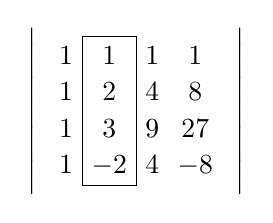
\begin{tikzpicture}
			\matrix(m)[
			matrix of math nodes,left delimiter=|,right delimiter=|,
			]
			{
		1 & 1  & 1 & 1  \\
		1 & 2  & 4 & 8  \\
		1 & 3  & 9 & 27 \\
		1 & -2 & 4 & -8 \\
			};  
			\draw (m-1-1.north east) rectangle (m-4-2.south east);
	\end{tikzpicture} \\
	=(-2-3)(-2-2)(-2-1)(3-2)(3-1)(2-1)
\end{array}
\] 

\subsubsection{X shape}

row and column exchange to move X to separate blocks. In conclusion, the result 
is the product of the determinants of the submatrices formed by the four 
elements lying on each arm of the X.
\[
	\begin{vmatrix}
		
	1  &   &   &   &   & 2 \\
	{} & 2 &   &   & 3 &   \\
     &   & 3 & 4 &   &   \\
     &   & 5 & 4 &   &   \\
     & 6 &   &   & 5 &   \\
	7  &   &   &   &   & 6 \\
	\end{vmatrix}
=
\begin{vmatrix}
	1 & 2 &   &   &   &   \\
	7 & 6 &   &   &   &   \\
    &   & 2 & 3 &   &   \\
    &   & 6 & 5 &   &   \\
    &   &   &   & 3 & 4 \\
    &   &   &   & 5 & 4 \\
\end{vmatrix}
=\prod \det B_i
=\!\!\!
\begin{array}{c}
	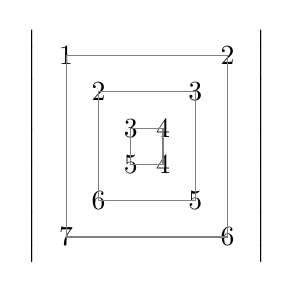
\begin{tikzpicture}
			\matrix(m)[
			matrix of math nodes,left delimiter=|,right delimiter=|,
			]
			{
	1 &   &   &   &   & 2 \\
    & 2 &   &   & 3 &   \\
    &   & 3 & 4 &   &   \\
    &   & 5 & 4 &   &   \\
    & 6 &   &   & 5 &   \\
	7 &   &   &   &   & 6 \\
			};
			\draw [draw=gray] (m-1-1) rectangle (m-6-6);
			\draw [draw=gray] (m-2-2) rectangle (m-5-5);
			\draw [draw=gray] (m-3-3) rectangle (m-4-4);
	\end{tikzpicture}
\end{array}
\] 
Odd order determinant is same method, with the center element alone acting as a
block of determinant. E.g.,
\[
	\begin{array}{c}
		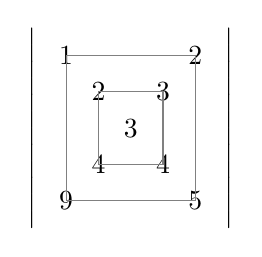
\begin{tikzpicture}
			\matrix(m)[
				matrix of math nodes,left delimiter=|,right delimiter=|,
			]
			{
				1 &   &   &   & 2 \\
          & 2 &   & 3 &   \\
          &   & 3 &   &   \\
          & 4 &   & 4 &   \\
				9 &   &   &   & 5 \\
			};
			\draw [draw=gray] (m-1-1) rectangle (m-5-5);
			\draw [draw=gray] (m-2-2) rectangle (m-4-4);
		\end{tikzpicture} \!\!\!
\end{array}
=(1\times 5-2\times9)(2\times4-3\times4)(3)
\] 

\subsubsection{Laplace}

\[
\begin{vmatrix}
	A & C \\
	O & B \\
\end{vmatrix}
=\begin{vmatrix}
	A & O \\
	C & B \\
\end{vmatrix}
=\begin{vmatrix}
	A & O \\
	O & B \\
\end{vmatrix}
=|A||B|
\] 
A is m order, B is n order
\[
\begin{vmatrix}
	C & A \\
	B & O \\
\end{vmatrix}
=\begin{vmatrix}
	O & A \\
	B & C \\
\end{vmatrix}
=\begin{vmatrix}
	O & A \\
	B & O \\
\end{vmatrix}
=(-1)^{mn}|A||B|
\] 

\subsubsection{Three diagonal}
\[
\Delta_n(a,b,c):=
\begin{vmatrix}
	b & c &  &  &  &  \\
	a & b & c &  &  &  \\
	 & a & b & \cdots  &  &  \\
	 &  & \vdots & \ddots & \vdots &  \\
	 &  &  & \cdots & a & b & c  \\
	 &  &  & & & a & b \\
\end{vmatrix}
\] 
\[
	\Delta_n=b\Delta_{n-1}-ac\Delta_{n-2}
\] 
the characteristic equation is
\[
\lambda^2 - b\lambda + ac = 0
\] 
We mainly care about the case below
\[
D_n=\Delta_n(\alpha,\alpha+\beta,\beta)=
\begin{vmatrix}
	\alpha+\beta & \beta &  &  &  &  \\
	\alpha & \alpha+\beta & \beta&  &  &  \\
	 & \alpha & \alpha+\beta & \cdots  &  &  \\
	 &  & \vdots & \ddots & \vdots &  \\
	 &  &  & \cdots  & \alpha+\beta & \beta  \\
	 &  &  &  & \alpha & \alpha+\beta \\
\end{vmatrix}
\] 
and\[
D_n=\Delta_n(1,\alpha+\beta,\alpha\beta)=
\begin{vmatrix}
	\alpha+\beta & \alpha\beta &  &  &  &  \\
	1 & \alpha+\beta & \alpha \beta&  &  &  \\
	 & 1 & \alpha+\beta & \cdots  &  &  \\
	 &  & \vdots & \ddots &  &  \\
	 &  &  &  & \alpha+\beta & \alpha\beta  \\
	 &  &  &  & 1 & \alpha+\beta \\
\end{vmatrix}
\] 
where both satisfy
\[
	\begin{align}
		D_1&=\alpha+\beta, \\
			 &=\frac{\alpha^2 - \beta^2}{\alpha - \beta} (\alpha \ne \beta)\\ 
		D_2&=(\alpha+\beta)^2 - \alpha\beta = \alpha^2 + \alpha\beta + \beta^2 \\
			 &=\frac{\alpha^3 - \beta^3}{\alpha - \beta} (\alpha \ne \beta)\\
	\end{align}
\] 
and $\alpha$ and $\beta$ acting as roots of the characteristic equation, so we 
can determine the cofficients of $D_n$ as follows:
\[
	D_n=
	\begin{cases}
		\frac{\alpha ^{n}-\beta^{n}}{\alpha - \beta} , & \alpha \ne \beta \\
		n\alpha^{n-1} , & \alpha = \beta
	\end{cases}
\]
\subsection{Cofactor/Minor sum questions}

If $\A$ is a square matrix, then the minor of the entry in the i-th
row and j-th column (also called the $(i, j)$ minor) is the determinant of the 
submatrix formed by deleting the i-th row and j-th column. This number is often 
denoted $M_{ij}$. The $(i, j)$ cofactor $C_{ij}$ is obtained by multiplying the minor by
$(-1)^{i+j}$.

\subsubsection{Use determinant to find cofactor/minor sum}

Example:
\[
	|A|=
	\begin{vmatrix}
		3 & 0  & 4  & 0 \\
		2 & 2  & 2  & 2 \\
		0 & -7 & 0  & 0 \\
		5 & 3  & -2 & 2 \\
	\end{vmatrix}
\] 

\textbf{Q1.} Find the sum of the cofactors of fourth row.

\[
	C_{41}+C_{42}+C_{43}+C_{44}
	= 
	\begin{vmatrix}
		3 & 0  & 4  & 0 \\
		2 & 2  & 2  & 2 \\
		0 & -7 & 0  & 0 \\
		1 & 1  & 1  & 1 \\
	\end{vmatrix}
\] 

\textbf{Q2.} Find the sum of the minors of fourth row.

\[
	\begin{align}
		 &M_{41}+M_{42}+M_{43}+M_{44} \\
		=&(-1)^{4+1}C_{41}+(-1)^{4+2}C_{42}+(-1)^{4+3}C_{43}+(-1)^{4+4}C_{44} \\
		=&-C_{41}+C_{42}-C_{43}+C_{44} \\
		=& \begin{vmatrix}
				3  & 0  & 4  & 0 \\
				2  & 2  & 2  & 2 \\
				0  & -7 & 0  & 0 \\
				-1 & 1  & -1 & 1 \\
			\end{vmatrix}
	\end{align}
\] 

\textbf{Q3.} Find $C_{41}-2C_{42}+C_{44}$

\[
	\begin{align}
		\text{ans}=& C_{41}+(-2)C_{42}+0C_{43}+C_{44} \\
		=&\begin{vmatrix}
				3  & 0  & 4  & 0 \\
				2  & 2  & 2  & 2 \\
				0  & -7 & 0  & 0 \\
				1  & -2 & 0  & 1 \\
			\end{vmatrix}
	\end{align}
\] 

\subsubsection{Cofactor sum when row sums equal constant}

When all row sums of matrix $\A$ equal a constant $k$ we can write
\[
\A \begin{bmatrix} 1 \\ 1 \\ \vdots \\ 1 \end{bmatrix}
= \begin{bmatrix} k \\ k \\ \vdots \\ k \end{bmatrix}
\] 
that is, the vector with all elements equal 1 is an eigenvector of $\A$,
which also acts as an eigenvector of $\A^{*}$ corresponding to the
eigenvalue $|A|/k$, thus
\[
	\A^{*} \begin{bmatrix}
		1 \\
		1 \\
		\vdots \\
		1
	\end{bmatrix} = \frac{|A|}{k} \begin{bmatrix}
		1 \\
		1 \\
		\vdots \\
		1
	\end{bmatrix}
\] 
and since
\[
	\A^{*} =
\begin{bmatrix}
	C_{11} & C_{21} & \dots & C_{n1} \\
	C_{12} & C_{22} & \dots & C_{n2} \\
	\vdots & \vdots & \ddots & \vdots \\
	C_{1n} & C_{2n} & \dots & C_{nn} 
\end{bmatrix}
\] 
we have
\[
	\sum_{i=1}^{n} C_{ij} = \frac{|A|}{k}
\] 
which says every column has the same sum of cofactors equal to $|A|/k$.

\textbf{Example:} 
Given 3 order matrix $\A$ satisfies $|A|=3$ and all
row sums equal 2, find the sum of the cofactors of the second column.

\textbf{Answer:} 3/2

\subsubsection{Sum of cofactors of diagonal elements}

\[
	\sum_{i=1}^{n} C_{ii} =\tr(\A^{*}) =
	\sum_{i=1}^n\frac{|A|}{\lambda_i}
\] 

\section{Matrix}

\begin{itemize}
	\item symmetric matrix: $\A=\A^T$
	\item anti-symmetric matrix: $\A=-\A^T$
\end{itemize}

Every square matrix can be uniquely decomposed into the sum of a symmetric
matrix and an anti-symmetric matrix:

\[
	\A = \frac{1}{2}(\A+\A^T) 
	+ \frac{1}{2}(\A-\A^T)
\] 
\subsection{Rank}

The rank of a matrix $\A$ can represent 
\begin{itemize}
	\item the maximum number of linearly independent rows or columns of $\A$
\end{itemize}

\subsubsection{Properties of rank}

Assume $\A$ is $m\times n$ matrix, and let $r(\A)$ denote the rank of $\A$.
\begin{itemize}
	\item $r(\A) = \dim \text{Col}(\A) = \dim \text{Row}(\A)$
	\item $r(\A) = r(\A^T) = r(\A\A^T) = r(\A^T\A)$
	\item $r(\A) \leq \min(m,n)$
	\item $r(\A\pm\B) \leq r(\A) + r(\B)$
	\item $r(\A\B) \leq \min(r(\A), r(\B))$
	\item $\max(r(\A), r(\B)) \leq
		r(\A | \B) \leq 
		r(\A) + r(\B)$
	\item $r(\A)=r(k\A)\quad(k\ne 0)$
	\item If $\boldsymbol{P},\boldsymbol{Q}$ are invertible matrices, then $
			r(\boldsymbol{A})=r(\boldsymbol{P}\A) = r(\A\boldsymbol{Q})
			= r(\boldsymbol{P}\A\boldsymbol{Q})
			$
	\item If $\A\B=\boldsymbol{0}$ then $r(\A)+r(\B) \leq n$
\end{itemize}

\subsubsection{Block matrix rank}

In general, we can use general row/column operations to simplify the block matrix
which do not change the rank of the matrix. Especially a row full rank block
can eliminate other blocks in the same row, and a column full rank block
can eliminate other blocks in the same column.(very useful when that block is
near to a zero block, then eliminate will not effect other blocks)

Here are some special cases:

For \textbf{row} block matrix:
\[(\A)=r(\A \vdots \A) = r(\A \vdots \A\B)\]
\[
	\left.\begin{align}
			r(\A+\B)\\ r(\A) \\ r(\B)
	\end{align}\right\} 
	\leq r(\A \vdots \B) \leq r(\A)+r(\B)
\] 

and when $\A$ is invertible or row full rank,
\[
	r(\A \vdots \B) = r(\A)
\]

For \textbf{column} block matrix:
\[
	r(\A)= r\begin{pmatrix} \A \\ \A \end{pmatrix}= r\begin{pmatrix} \A \\ \B\A \end{pmatrix}
\]
\[
		\left.\begin{align}
				r(\A+\B)\\ r(\A) \\ r(\B)
		\end{align}\right\} 
		\leq r\begin{pmatrix} \A \\ \B \end{pmatrix} \leq r(\A)+r(\B)
		\]

and when $\A$ is invertible or column full rank, 
\[
	r\begin{pmatrix} \A \\ \B \end{pmatrix} = r(\A)
\]

For \textbf{diag blocks} matrix:
\[
	r\begin{pmatrix} \A & O \\
		O & \B \\ \end{pmatrix}
	=
	r\begin{pmatrix} O & \A \\
	\B & O \\ \end{pmatrix}
	= r(\A) + r(\B)
\] 

For \textbf{mixed blocks} matrix:
\[
	r(\A)+r(\B)+r(\boldsymbol{C})
	\geq
	r\begin{pmatrix} \A & O \\
		\boldsymbol{C}& \B \\ \end{pmatrix}
	\geq
	r(\A)+r(\B)
\] 
\[
	r(\A)+r(\B)+r(\boldsymbol{D})
	\geq
	r\begin{pmatrix} \A & \boldsymbol{D} \\
		O & \B \\ \end{pmatrix}
	\geq
	r(\A)+r(\B)
\] 

when $\boldsymbol{C}$ or $\boldsymbol{D}$ are listed below, we have:
\[
\begin{align}
	r\begin{pmatrix} \A & \A\boldsymbol{C} \\
			O & \B \\ \end{pmatrix}
	= r(\A)+r(\B) \\
	r\begin{pmatrix} \A & \boldsymbol{D}\B \\
			O & \B \\ \end{pmatrix}
	= r(\A)+r(\B) \\
		r\begin{pmatrix} \A & \A \\
				O & \B \\ \end{pmatrix}
	= r\begin{pmatrix} \A & \B \\
				O & \B \\ \end{pmatrix}
	= r(\A)+r(\B) \\
\end{align}
\] 


\subsubsection{Rank 1 matrix}

Rank equals to one means the maximal linearly independent rows or columns is one,
thus all rows are multiples of the one column $\boldsymbol{\alpha}$ (always choose the simplest non-zero 
column and call it the key column), and other columns are multiples of $\boldsymbol{\alpha}$ 
we use the corresponding multiples to form the row vector $\boldsymbol{\beta}^T$
(choose non-zero row). And sometimes we call $\boldsymbol{\beta}^T$ the coefficient vector.

So a rank 1 matrix can be written as the product of a column vector and a row vector:
\[
	\A = \boldsymbol\alpha \boldsymbol\beta^T
\]

and we have
\[
\tr(\A) = \boldsymbol\beta^T \boldsymbol\alpha = \boldsymbol\alpha^T \boldsymbol\beta
\] 

also it has simple eigenvalues and eigenvectors, since $\A \boldsymbol{\alpha} =  \boldsymbol{\alpha} (
\boldsymbol{\beta}^T \boldsymbol{\alpha})=\tr(\A)\boldsymbol{\alpha}$, one
eigenvalue is $\tr(\A)$, and the corresponding eigenvector is $\boldsymbol{\alpha}$.
It can be verified that other eigenvalues are all zero, $\boldsymbol{\beta}\neq\boldsymbol{0}$
give $\dim\text{Nul}\ \boldsymbol{\beta}^{T}=n-1$, which means there exist $n-1$ linearly
independent vectors $\boldsymbol{v}_1, \boldsymbol{v}_2, \dots, \boldsymbol{v}_{n-1}$ 
(one choice of basis of the null space of $\boldsymbol{\beta}^{T}$)
satisfying $\boldsymbol{\beta}^{T}\boldsymbol{v}_i=0$, also
$\A \boldsymbol{v}_i = \boldsymbol{\alpha}( \boldsymbol{\beta}^{T}\boldsymbol{v}_i)
=\boldsymbol{0}$, so the other $n-1$ eigenvalues are all zero,
and the corresponding eigenvectors are $\boldsymbol{v}_1, \boldsymbol{v}_2, \dots, \boldsymbol{v}_{n-1}$.

When $\tr(\A)=0$, all eigenvalues are zero. $\boldsymbol{\alpha}$ is still an eigenvector,
but it falls into the null space, so there are only $n-1$ linearly independent eigenvectors.
Otherwise, there are $n$ linearly independent eigenvectors, which means
$\A$ is diagonalizable, so we have
\[
	\A \text{ is diagonalizable} \iff \tr(\A) \ne 0
	\quad(\text{when } \rank(\A)=1)
\]

It is also easy to calculate powers of rank 1 matrix:
\[
	\A^n = (\boldsymbol\alpha \boldsymbol\beta^T)^n
	= \boldsymbol{\alpha}\boldsymbol{\beta}^T\boldsymbol{\alpha}\boldsymbol{\beta}^T \cdots
	\boldsymbol{\alpha}\boldsymbol{\beta}^T
	= \boldsymbol{\alpha}(\boldsymbol{\beta}^T\boldsymbol{\alpha})^{n-1} \boldsymbol{\beta}^T
	= \tr(\A)^{n-1}\A
\]

\textbf{Example:}
\[
	\A=
\begin{bmatrix}
	2 & 4 & 6 \\
	1 & 2 & 3 \\
	3 & 6 & 9 \\
\end{bmatrix}
=
\begin{bmatrix} 2\\ 1\\ 3\\ \end{bmatrix}
\begin{bmatrix} 1 & 2 & 3 \\ \end{bmatrix}
\] 
\[ \tr(\A) = 2+2+9 = 2\times 1 + 1\times 2 + 3\times 3 \] 

Eigenvalues are 13,0,0; eigenvectors are
\[
\begin{bmatrix} 2\\ 1\\ 3\\ \end{bmatrix},
\begin{bmatrix} -2\\ 1\\ 0\\ \end{bmatrix},
\begin{bmatrix} -3\\ 0\\ 1\\ \end{bmatrix}
\]


\subsection{Adjugate}

\begin{itemize}
	\item $\A\A^{*} = \A^{*}\A =
		|A|\I$ \\
		When $|A| \ne 0$ we have
		\[
			\A^{-1} = \frac{1}{|A|}\A^{*}
			,\quad
			\A^{*} = |A|\A^{-1}
		\] 
	\item $(k\A)^{*} = k^{n-1}\A^{*}$
		\quad (derived directly from last property)
	\item $(\A^T)^{*} = (\A^{*})^T$
	\item $(\A\B)^{*} = \B^{*}\A^{*}$
	\item $|\A^{*}| = |A|^{n-1}$
	\item $(\A^{-1})^{*}=(\A^{*})^{-1}=\dfrac{
		\A}{|A|}$
	\item $(\A^{*})^{*} = |A|^{n-2}\A$
	\item $\rank(\A^{*})=
		\begin{cases}
			n,\quad \rank(\A)=n \\
			1,\quad \rank(\A)=n-1 \\
			0,\quad \rank(\A)<n-1 \\
		\end{cases}$

		
\end{itemize}

\subsubsection{Block matrix adjugate}

Here $\A$ is m by m, $\B$ is n by n invertible matrix.
\[
\begin{align}
	&
	\begin{pmatrix} A & C \\
		O & B \\ \end{pmatrix}^{*}
	=
	\begin{vmatrix} A & C \\
		O & B \\ \end{vmatrix}
	\begin{pmatrix} A & C \\
	O & B \\ \end{pmatrix}^{-1}
	=|A||B|
	\begin{pmatrix} A^{-1} & -A^{-1}CB^{-1} \\
		O & B^{-1} \\ \end{pmatrix}
	=\begin{pmatrix}
		|B|A^{*} & -A^{*}C B^{*} \\
		O & |A|B^{*} \\
	\end{pmatrix} \\
  &
		\begin{pmatrix} A & O \\
		C & B \\ \end{pmatrix}^{*}
	=
	\begin{vmatrix} A & O \\
		C & B \\ \end{vmatrix}
	\begin{pmatrix} A & O \\
	C & B \\ \end{pmatrix}^{-1}
	=|A||B|
	\begin{pmatrix} A^{-1} & O \\
		-B^{-1}CA^{-1} & B^{-1} \\ \end{pmatrix}
	=\begin{pmatrix}
		|B|A^{*} & O \\
		-B^{*}C A^{*} & |A|B^{*} \\
	\end{pmatrix}
\end{align}
\] 
\[
\begin{align}
	&
		\begin{pmatrix} C & A \\
		B & O \\ \end{pmatrix}^{*}
	=
	\begin{vmatrix} C & A \\
		B & O \\ \end{vmatrix}
	\begin{pmatrix} C & A \\
	B & O \\ \end{pmatrix}^{-1}
	=(-1)^{mn}|A||B|
	\begin{pmatrix} O & B^{-1} \\
		A^{-1} & -A^{-1}CB^{-1} \\ \end{pmatrix}
	=(-1)^{mn}
	\begin{pmatrix} O & |A|B^{*} \\
		|B|A^{*} & -A^{*}C B^{*} \\ \end{pmatrix} \\
	&
	\begin{pmatrix} O & A \\
	B & C \\ \end{pmatrix}^{*}
	=
	\begin{vmatrix} O & A \\
	B & C \\ \end{vmatrix}
	\begin{pmatrix} O & A \\
	B & C \\ \end{pmatrix}^{-1}
	=(-1)^{mn}|A||B|
	\begin{pmatrix} -B^{-1}CA^{-1} & B^{-1} \\
		A^{-1} & O \\ \end{pmatrix}
	=(-1)^{mn}
	\begin{pmatrix} -B^{*}C A^{*} & |A|B^{*} \\
		|B|A^{*} & O \\ \end{pmatrix}
\end{align}
\] 

Tips to remember:
\begin{itemize}
	\item First write down the diagonal(or secondary diagonal) block 
		$(A,B)\rightarrow(|B|A^{*},|A|B^{*})$
	\item The O block remains O
	\item The other two blocks are negative of the product of the two
		adjugates and the C block, to remember the order of multiplication,
		\subitem The left of C is same as row
		\[
			\begin{pmatrix} |B|\boxed{A^{*}} & -\boxed{A^{*}}C B^{*} \\
				O & |A|B^{*} \\ \end{pmatrix} \\
			\begin{pmatrix} O & |A|B^{*} \\
				\boxed{B^{*}}|A^{*}| & -\boxed{B^{*}}C A^{*} \\ \end{pmatrix}
		\] 
		\subitem The right of C is same as column
		\[
			\begin{pmatrix} O & \hspace{14pt} |A|\boxed{B^{*}} \\
				|B|A^{*} & -A^{*}C \boxed{B^{*}} \\ \end{pmatrix} \\
				\begin{pmatrix} -B^{*}C \boxed{A^{*}} & |A|B^{*} \\
				\hspace{15pt}|B|\boxed{A^{*}} & O \\ \end{pmatrix}
		\] 
\end{itemize}

\subsection{Inverse}

\subsubsection{$\A^{-1}\B$ and $\B\A^{-1}$}

\begin{itemize}
	\item $\A^{-1}\B$ is row operation make $\A$
	to identity matrix: (left multiplication corresponds to row operation)
		\[
			(\A | \B) \sim
			(\I | \A^{-1}\B)
		\] 
	\item $\B\A^{-1}$ is column operation make $\A$
	to identity matrix: (right multiplication corresponds to column operation)
		\[
			\begin{pmatrix}
				\A \\
				\B \\
			\end{pmatrix} \sim
			\begin{pmatrix}
				\I \\
				\B\A^{-1} \\
			\end{pmatrix}
		\]
\end{itemize}

We mainly care about this method's complexity on 3 order matrix in order to compare
with other methods. Column operation is similar to row operation, so we only analyze
row operation here.

First to eliminate the first column below the first row: 
 \[
	 \left( \begin{array}{ccc|ccc}
		a_{11} & a_{12} & a_{13} &  1 & 0 & 0 \\
		a_{21} & a_{22} & a_{23} &  0 & 1 & 0 \\
		a_{31} & a_{32} & a_{33} &  0 & 0 & 1 \\
	\end{array}\right)
	\rightarrow
	\left( \begin{array}{ccc|ccc}
		a_{11} & a_{12} & a_{13} &  1 & 0 & 0 \\
		0      & b_{22} & b_{23} &  m_{21} & 1 & 0 \\
		0      & b_{32} & b_{33} &  m_{31} & 0 & 1 \\
	\end{array} \right)
\] 
each row cost 1 multiplications to get the multiplier, 2 multiplications to get
subtracted items, and so 2 subtractions(for the first step, operation on $\I$ is
too simple to count), so
the first step 2 rows totally cost \underline{6 multiplications and 4 subtractions}.

Second to eliminate the second column below the second row:
 \[
	 \left( \begin{array}{ccc|ccc}
		a_{11} & a_{12} & a_{13} &  1 & 0 & 0 \\
		0      & b_{22} & b_{23} &  m_{21} & 1 & 0 \\
		0			& 0      & c_{33} &  n_{31} & n_{32} & 1 \\
	\end{array}\right)
\]
cost 1 multiplication to get the multiplier, 2 multiplications to get
subtracted items, and 3 subtractions, so the second step costs 
\underline{2 multiplications and 3 subtractions.}

Make the diagonal elements 1, cost \underline{9 multiplications.}

To eliminate the third column above the third row:
 \[
	 \left( \begin{array}{ccc|ccc}
			 1 & d_{12} & d_{13} &  e_{11} & 0 & 0 \\
			 0 & 1      & d_{23} &  e_{21} & e_{22} & 0 \\
			 0 & 0      & 1			&  f_{31} & f_{32} & f_{33} \\
		 \end{array}\right) \rightarrow
	 \left( \begin{array}{ccc|ccc}
			 1 & d_{12} & 0 &  g_{11} & g_{12} & g_{13} \\
			 0 & 1      & 0 &  g_{21} & g_{22} & g_{23} \\
			 0 & 0      & 1 &  f_{31} & f_{32} & f_{33} \\
	 \end{array}\right)
 \]
1 multiplication 1 subtraction per element, totally \underline{3 multiplications and 3 subtractions}
(need operate on $ e_{11}, e_{21}, e_{22} $).
To eliminate the second column above the second row, cost \underline{3 multiplications and 3 subtractions.}
In total, the whole process costs
\[
	\boxed{
	23 \text{ multiplications and } 13 \text{ subtractions.}
}
\]

\subsubsection{Use adjugate to find inverse}

2 order matrix:
\[
\A=\begin{bmatrix}
	a & b \\
	c & d \\
\end{bmatrix}
\]
then
\[
	\A^{*} =\begin{bmatrix}
	d & -b \\
	-c & a \\
	\end{bmatrix}
\]
and
\[
	\A^{-1} = \frac{1}{|A|}\A^{*} =
	\frac{1}{ad-bc}\begin{bmatrix}
	d & -b \\
	-c & a \\
	\end{bmatrix}
\] 

3 order matrix:

\subsubsection{Block matrix inverse}

\[
\begin{bmatrix}
	A & O \\
	O & B \\
\end{bmatrix}^{-1}
=
\begin{bmatrix}
	A^{-1} & O \\
	O & B^{-1} \\
\end{bmatrix}
\] 
\[
\begin{bmatrix}
	O & A \\
	B & O \\
\end{bmatrix}^{-1}
=
\begin{bmatrix}
	O & B^{-1} \\
	A^{-1} & O \\
\end{bmatrix}
\] 

\subsubsection{Can decomposed to rank 1 matrix plus $k\I$}

If $\A$ can be decomposed to $\A=\boldsymbol\alpha \boldsymbol\beta^T + k\I$,
let $\boldsymbol{R}=\boldsymbol{\alpha} \boldsymbol{\beta}^T$, then
\[
	\boldsymbol{R}^2=\tr(\boldsymbol{R})\boldsymbol{R}=
	(\A-k\I)^2
\] 
substitute $\boldsymbol{R}=\A-k\I$ and rearrange we have
\[
	\begin{align}
	\A^2 - (2k+\tr(\boldsymbol{R}))\A + (k^2 + k\ \tr(\boldsymbol{R}))\I = \boldsymbol{O} \\
	\A(\A - (2k+\tr(\boldsymbol{R}))\I) = -(k^2 + k\ \tr(\boldsymbol{R}))\I \\
	\end{align}
\] 
\[
	\A^{-1} = \frac{
		\A - (2k+\tr(\boldsymbol{R}))\I
	}{
		-(k^2 + k\ \tr(\boldsymbol{R}))
	}
\] 

Also it can be written as below using $ \boldsymbol{A}=\boldsymbol{R} + k\I $
\[
	\A^{-1} = \frac{1}{k}\left(\I-\frac{\boldsymbol{R}}{k+\tr(\boldsymbol{R})}\right)
\] 

In fact, this is a special case of Sherman-Morrison formula.
\[
	(\boldsymbol{A} + \boldsymbol{u}\boldsymbol{v}^T)^{-1} =
	\boldsymbol{A}^{-1} -
	\frac{
		\boldsymbol{A}^{-1}\boldsymbol{u}\boldsymbol{v}^T\boldsymbol{A}^{-1}
	}{
		1 + \boldsymbol{v}^T\boldsymbol{A}^{-1}\boldsymbol{u}
	}
\] 

Now analyze the complexity of this method on 3 order matrix:

To test $k$, use the method we talked at the beginning of this document, cost
a two order determinant, and one division, in total needs \underline{3 multiplications and
1 subtraction}, and subtract $k\I$ from $\A$, cost \underline{3 subtractions.}
when test passed, calculate $\tr(\boldsymbol{R})+k$, cost \underline{2 additions 1 multiplication.}
To get $\boldsymbol{R}/(...)$ needs \underline{9 multiplications.}
Then sub from $\I$ need {3 subtractions}. In common we don't need to multiply $1/k$
to get the final result, so we skip this step.
In total, this method costs
\[
	\boxed{
		13 \text{ multiplications and } 5 \text{ subtractions.}
	}


\section{Power of matrix}

In general, to calculate $\A^{n}$ we can use diagonalization method:
\[
	\A = \boldsymbol{P} \boldsymbol{\Lambda} \boldsymbol{P}^{-1} \quad \Rightarrow \quad
	\A^{n} = \boldsymbol{P} \boldsymbol{\Lambda}^{n} \boldsymbol{P}^{-1}
\]

\subsection{3 $\times$ 3 Triangular matrix with same diagonal elements}

If $\A$ is an upper or lower triangular matrix with all diagonal elements equal to $k$,
then we can write $\A$ as
\[
	\A = k\I + \B
\]
and calculate its power as
\[
	\A^{n} = (k\I + \B)^{n} =
	\sum_{i=0}^{n} \binom{n}{i} (k\I)^{n-i} \B^{i} =
	\sum_{i=0}^{n} \binom{n}{i} k^{n-i} \B^{i}
\] 
where $\B$ is a strictly upper or lower triangular matrix.(triangular matrix 
with all diagonal elements equal to zero) Although $\B^{i}$ not easy to calculate,
For 3 order matrix, we have quick method to calculate $\B^{2}$
\[
	\B =
\begin{bmatrix}
	0 & a & b \\
	0 & 0 & c \\
	0 & 0 & 0 \\
\end{bmatrix}
\quad \Rightarrow \quad
\B^{2} =
\begin{bmatrix}
	0 & 0 & ac \\
	0 & 0 & 0 \\
	0 & 0 & 0 \\
\end{bmatrix}
\]
And since $\B^{3}=\boldsymbol{O}$, we have
\[
	\A^{n} = k^{n}\I + nk^{n-1}\B + \frac{n(n-1)}{2}k^{n-2}\B^{2}
\]
When $k=1$, we have
\[
	\A^{n} = \I + n\B + \frac{n(n-1)}{2}\B^{2}
\]
In matrix form:
\[
	\begin{bmatrix}
		1 & a & b \\
      & 1 & c \\
      &   & 1 \\
	\end{bmatrix}^{n} =
\begin{bmatrix}
	1 & na & nb + \frac{n(n-1)}{2} ac \\
			& 1 & nc \\
			&   & 1 \\
\end{bmatrix}
\] 
Although the derivation is assume n is a positive integer, the final result
holds for any integer n, and we have an inverse formula:
\[
	\begin{bmatrix}
		1 & a & b \\
      & 1 & c \\
      &   & 1 \\
	\end{bmatrix}^{-1} =
	\begin{bmatrix}
		1 & -a & - b +ac \\
			& 1 & -c \\
			&   & 1 \\
	\end{bmatrix}
\] 



\subsection{Block matrix power}
\[
\begin{bmatrix}
	A & O \\
	O & B \\
\end{bmatrix}^{n}
=
\begin{bmatrix}
	A^{n} & O \\
	O & B^{n} \\
\end{bmatrix}
\] 

\section{Solution of linear system}

\subsection{properties of solution}

If $\boldsymbol{\psi}_1, \boldsymbol{\psi}_2, \dots, \boldsymbol{\psi}_s$ are solutions
of $\A \boldsymbol{x}=\boldsymbol{b}$, let $\boldsymbol{\Psi}=(\boldsymbol{\psi}_1, \boldsymbol{\psi}_2, \dots, \boldsymbol{\psi}_s)$,
then for any linear combination of $\boldsymbol{\psi}_i$ 
\[
\boldsymbol{y} = \sum_{i=1}^{s} k_i \boldsymbol{\psi}_i= \boldsymbol{\Psi} \boldsymbol{k}
\] 
has the following result 
\[ \A \boldsymbol{y} = \A \boldsymbol{\Psi} \boldsymbol{k}
= \boldsymbol{b}\boldsymbol{1}_{1\times s} \boldsymbol{k}
= \left(\sum_{i=1}^{s} k_i\right) \boldsymbol{b} \]
thus we have the following properties:
\begin{equation}
\sum_{i=1}^{s} k_i \boldsymbol{\psi}_i
\text{ is a solution of } \A \boldsymbol{x}=0 \iff \sum_{i=1}^{s} k_i = 0
\label{eq:nohomo_sols_s0}
\end{equation}
\begin{equation}
	\sum_{i=1}^{s} k_i \boldsymbol{\psi}_i
\text{ is a solution of } \A \boldsymbol{x}=\boldsymbol{b} \iff \sum_{i=1}^{s} k_i = 1
\label{eq:nohomo_sols_s1}
\end{equation}
Example: If $\boldsymbol{\psi}_1, \boldsymbol{\psi}_2$ are two solutions
of $\A \boldsymbol{x}=\boldsymbol{b}$, then
\begin{itemize}
	\item $(\boldsymbol{\psi}_1 - \boldsymbol{\psi}_2)/2$ is a solution of $\A \boldsymbol{x}=0$
	\item $(\boldsymbol{\psi}_1 + \boldsymbol{\psi}_2)/2$ is a solution of $\A \boldsymbol{x}=\boldsymbol{b}$
\end{itemize}

\end{document}
